\documentclass[xcolor=dvipsnames,beamer]{beamer} %handout,notes=show

\usepackage{textcomp}
\usepackage[utf8]{inputenc}
% \usepackage{default}
\usepackage{graphicx}
%  \usepackage[pdftex]{hyperref}
\usepackage{url}
\usepackage{amsmath}

% frames have to be fragile
\newif\ifnotes
% \notestrue

%\notestrue


\ifnotes
%\setbeamertemplate{note page}[plain]
\setbeamertemplate{note page}[compress]
\setbeamerfont{note page}{size=\large}
\setbeameroption{show only notes}
%\setbeameroption{show notes}
\usepackage{pgfpages}
\pgfpagesuselayout{2 on 1}[a4paper,border shrink=5mm]%
\else
%\setbeameroption{hide notes}
\fi
%\notesfalse



% nastaveni TypeWriter
%\usepackage{courier}
%\usepackage{lmodern}
%\renewcommand*\ttdefault{txtt}
\DeclareFontShape{OT1}{cmtt}{bx}{n}{<5><6><7><8><9><10><10.95><12><14.4><17.28><20.74><24.88>cmttb10}{}


% \usepackage{verbatim}
\usepackage[absolute,overlay]{textpos}

\usepackage{listings}
% \usepackage{courier}
\definecolor{grey}{RGB}{70,70,70}
\definecolor{green}{RGB}{0,255,0}
\definecolor{red}{RGB}{202,53,53}
\definecolor{lightGrey}{RGB}{250,250,250}
\definecolor{darkGrey}{RGB}{50,50,50}


\usepackage{color}
\definecolor{lightgray}{rgb}{.9,.9,.9}
\definecolor{darkgray}{rgb}{.4,.4,.4}
\definecolor{purple}{rgb}{0.65, 0.12, 0.82}


% \usetheme{Warsaw}
\usetheme{Madrid}
% \usetheme{Szeged}
% \useoutertheme{infolines}
% \usecolortheme[named=MidnightBlue]{structure}
\usecolortheme[named=PineGreen]{structure}
% \setbeamertemplate{navigation symbols}{}




\title[HPC benchmarking ET models OSGEO]
{Big data ET models \& benchmarking\\
with distributed OSGEO tools}
%\subtitle{SVO\v{C}}
%\pdforstring{}{}
\author[Yann Chemin]
{\vspace{50pt}\\
Yann Chemin}

\institute[IWMI]
{International Water Management Institute\\
 \vspace{5pt}
\begin{flushleft}
 \includegraphics[width=14cm]{ciacanolafield}
\end{flushleft}
}
\date{\tiny November 2nd, 2013}


%\AtBeginSection[]{\begin{frame}\frametitle{Obsah}%
%\tableofcontents[currentsection ]\end{frame}}
%\AtBeginSubsection[]
%{
%  \begin{frame}<beamer>
%  \frametitle{Obsah}
%  \tableofcontents[currentsection,currentsubsection]
%  \end{frame}
%}

\setbeamercovered{transparent}

\hypersetup{%
	pdfauthor={Yann Chemin},%
	pdfsubject={Presentation},%
    pdfkeywords={HPC, benchmarking, Evapotranspiration, models, OSGEO}
}

\usepackage{listings}
\lstdefinestyle{C++}{%
  % language
  language=C++, % [ANSI]C++, GNU, ISO, Visual
  basicstyle=\ttfamily\small,
  commentstyle=\itshape,
  keywordstyle=\bfseries, % needs another \ttdefault
  showstringspaces=false,
  stringstyle=,
  identifierstyle=,
  % working with latex
  escapeinside={//lst}{\^^M}  
}

\lstset{%
%  frame=trBL,
%  backgroundcolor=\color{},
  linewidth=\textwidth,
  % working with latex
  gobble=2,
  % float
  nolol=false,
  numberbychapter=true,
  captionpos=t,% tb
  % breaking lines
  breaklines=true,
  breakatwhitespace=true,
  breakindent=10em,
  breakautoindent=true,
  prebreak={},
  postbreak={},
  %document default style
    basicstyle=\ttfamily
}


%\lstlistlistingname % The header name for the list of listings.
%\lstlistingname % The caption label for listings.

\lstnewenvironment{cmdline}[1][]
{\lstset{
  style=C++,
  #1}}
{}

\lstnewenvironment{scpp}[1][]
{\lstset{
  style=C++,
  #1}}
{}

\lstnewenvironment{ncpp}[1][]
{\lstset{
  style=C++,
  numbers=left, 
  numberstyle=\scriptsize, 
  stepnumber=1,
  numbersep=5pt,
  #1}}
{}

\lstnewenvironment{fcpp}[1][]
{\lstset{
  style=C++,
  float,
   % line numbers
  numbers=left, 
  numberstyle=\scriptsize, 
  stepnumber=1,
  numbersep=5pt,
  #1}}
{}


\lstnewenvironment{lcpp}[1][]
{\lstset{%
style=C++,
numbers=left, 
numberstyle=\scriptsize, 
stepnumber=1,
numbersep=5pt,
xleftmargin=12pt,
breakautoindent=false,
breaklines=false,%
#1}}{}

\lstnewenvironment{smallcpp}[1][]
{\lstset{%
style=C++,
numbers=left, 
numberstyle=\tiny, 
stepnumber=1,
numbersep=5pt,
xleftmargin=12pt,
breakautoindent=false,
breaklines=false,%
basicstyle=\ttfamily\scriptsize,
#1}}{}


\lstnewenvironment{pscpp}[1][]
{\lstset{%
style=C++,
xleftmargin=12pt,
breakautoindent=false,
breaklines=false,
#1}}{}


%\lstset{index={square},index={[2]root}}


\newcommand{\overovaciref}[1]{{\scriptsize(\ref{#1})}}


\usepackage{tipa}
\newcommand{\pron}[2]{#1 [#2]}

%%%%%%%%%%%%%%%%%%%%%%%%%%%%%%%%%%%%%%%%%%%%%%%%%%%%%%%%%%%%%%%%%%%%
% TOC frame setup
%%%%%%%%%%%%%%%%%%%%%%%%%%%%%%%%%%%%%%%%%%%%%%%%%%%%%%%%%%%%%%%%%%%%
\usepackage{multicol}
\colorlet{mycolor}{orange!80!black}% change this color to suit your needs
\AtBeginSection[]{
  \setbeamercolor{section in toc shaded}{use=structure,fg=structure.fg}
  \setbeamercolor{section in toc}{fg=mycolor}
  \setbeamercolor{subsection in toc shaded}{fg=black}
  \setbeamercolor{subsection in toc}{fg=mycolor}
  \frame<beamer>{\begin{multicols}{2}
  \frametitle{Outline}
  \setcounter{tocdepth}{2}  
  \tableofcontents[currentsection,subsections]
\end{multicols} 
 }
}

\setbeamercolor{author in head/foot}{fg=white}
\setbeamercolor{title in head/foot}{fg=white}
\setbeamercolor{section in head/foot}{fg=mycolor}
\setbeamertemplate{section in head/foot shaded}{\color{white!70!black}\insertsectionhead}
\setbeamercolor{subsection in head/foot}{fg=mycolor}
\setbeamertemplate{subsection in head/foot shaded}{\color{white!70!black}\insertsubsectionhead}
\setbeamercolor{frametitle}{fg=white}
\setbeamercolor{framesubtitle}{fg=white}

%%%%%%%%%%%%%%%%%%%%%%%%%%%%%%%%%%%%%%%%%%%%%%%%%%%%%%%%%%%%%%%%%%%%
%%%%%%%%%%%%%%%%%%%%%%%%%%%%%%%%%%%%%%%%%%%%%%%%%%%%%%%%%%%%%%%%%%%%
%%%%%%%%%%%%%%%%%%%%%%%%%%%%%%%%%%%%%%%%%%%%%%%%%%%%%%%%%%%%%%%%%%%%
\begin{document}

%%%%%%%%%%%%%%%%%%%%%%%%%%%%%%%%%%%%%%%%%%%%%%%%%%%%%%%%%%%%%%%%%%%%
\begin{frame}
 \maketitle
\end{frame}
%%%%%%%%%%%%%%%%%%%%%%%%%%%%%%%%%%%%%%%%%%%%%%%%%%%%%%%%%%%%%%%%%%%%


%%%%%%%%%%%%%%%%%%%%%%%%%%%%%%%%%%%%%%%%%%%%%%%%%%%%%%%%%%%%%%%%%%%%
\begin{frame}{Contents}
 \begin{multicols}{2}
  \setcounter{tocdepth}{2}  
  \tableofcontents
 \end{multicols} 
\end{frame}
%%%%%%%%%%%%%%%%%%%%%%%%%%%%%%%%%%%%%%%%%%%%%%%%%%%%%%%%%%%%%%%%%%%%


%%%%%%%%%%%%%%%%%%%%%%%%%%%%%%%%%%%%%%%%%%%%%%%%%%%%%%%%%%%%%%%%%%%%
\begin{frame}[fragile]{CGIAR}

Consultative Group for International Agricultural Research\\
Ratified on October 2nd, 2013\\
Full Open Access \& Open Source research data and publication
\newline

\begin{columns}[l]
\column{0.5\textwidth}
\begin{center}
\begin{itemize}
 \item International Public Goods
 \item Public Domain
 \item Publications Open Access
 \item FOSS models and algorithms
\end{itemize}
\end{center}

\column{0.5\textwidth}
\begin{center}
  
\includegraphics[width=1.5cm]{CGIAR_Green}
  \hspace{5mm}
  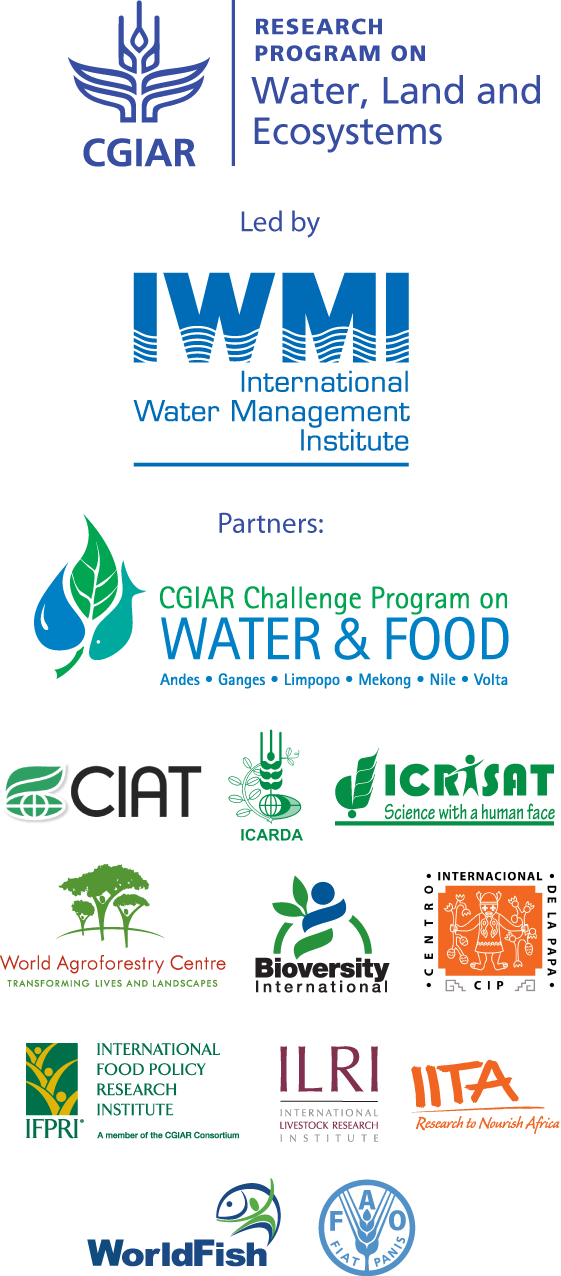
\includegraphics[width=1.8cm]{WLE_and_partners-vertical_logo_strip.png}
\end{center}
\end{columns}
\vspace{5mm} 2018: all 15 CG centres, already FOSS4G Lab:
(\href{http://gsl.worldagroforestry.org}{gsl.worldagroforestry.org})
\end{frame}


\section{Introduction}
%%%%%%%%%%%%%%%%%%%%%%%%%%%%%%%%%%%%%%%%%%%%%%%%%%%%%%%%%%%%%%%%%%%%
\begin{frame}[fragile]{Introduction}

Evapotranspiration is the largest transiting quantity in the daily 
hydrological cycle along with rain. It is used by scientists and
managers in:
\newline\linebreak

\begin{itemize}
 \item Irrigation systems performance
 \item Crop water productivity
 \item Water accounting
 \item Wetlands-agriculture interface
 \item Basin water uses quantification
 \item Climate change on water cycle \& users
\end{itemize}
\end{frame}

\section{Evapotranspiration Modeling}
%%%%%%%%%%%%%%%%%%%%%%%%%%%%%%%%%%%%%%%%%%%%%%%%%%%%%%%%%%%%%%%%%%%%
\begin{frame}[fragile]{Overview}

There are several types of evapotranspiration modeling methods:\\

\begin{itemize}
 \item Reference ET: Hargreaves, Penman-Monteith
 \item Potential ET: Priestley-Taylor, astronomical
 \item Actual ET: Thermodynamic/energy balance (mostly)
\end{itemize}

\begin{block}{OSGEO tools}
\begin{columns}[l]
\column{0.2\textwidth}
\begin{center}

\includegraphics[width=2cm]{OSGeo_logo}
\end{center}
\column{0.4\textwidth}
\begin{center}
\includegraphics[width=2cm]{GDALLogoColor}
\end{center}
\column{0.4\textwidth}
\begin{center}

\includegraphics[width=2cm]{Grass_GIS}
\end{center}
\end{columns}
\end{block}
\end{frame}

\subsection{ET \& Equity in Irrigation}
%%%%%%%%%%%%%%%%%%%%%%%%%%%%%%%%%%%%%%%%%%%%%%%%%%%%%%%%%%%%%%%%%%%%
\begin{frame}[fragile]{Equity of water use in irrigation systems}

Irrigation water monitoring \& management
\begin{itemize}
 \item Map: Uniform colour is equity of water distribution
 \item Graph: Irrigation system equity in time (mm/d, daily, 12 years)
\end{itemize}

\begin{columns}[l]
\column{0.2\textwidth}
\begin{center}
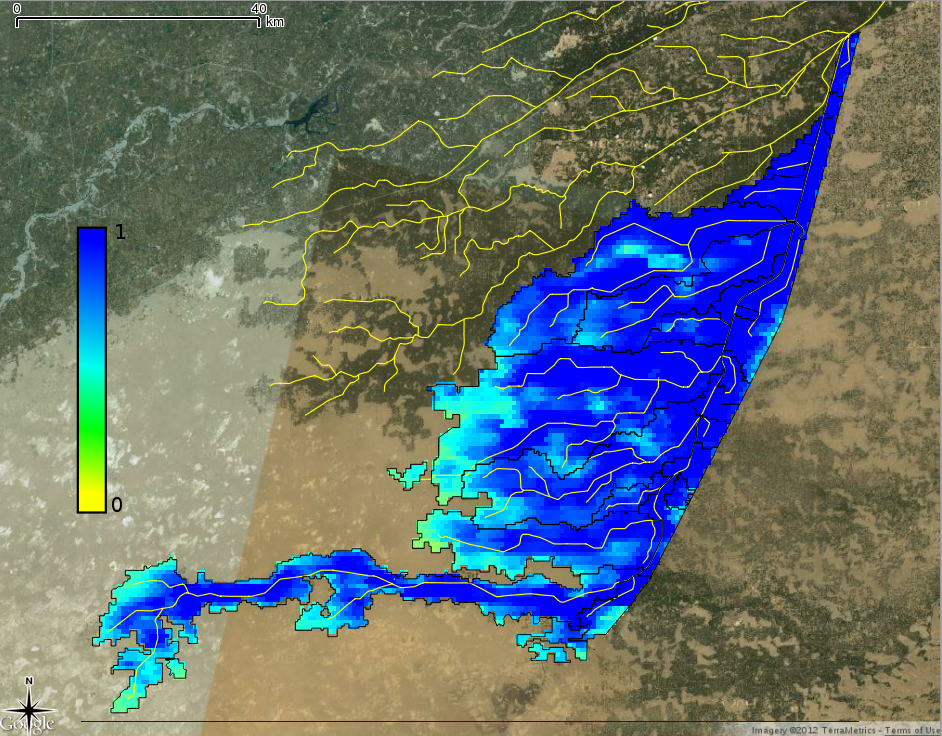
\includegraphics[width=4cm]{fess2012ef}
\end{center}

\column{0.8\textwidth}
\begin{flushright}
  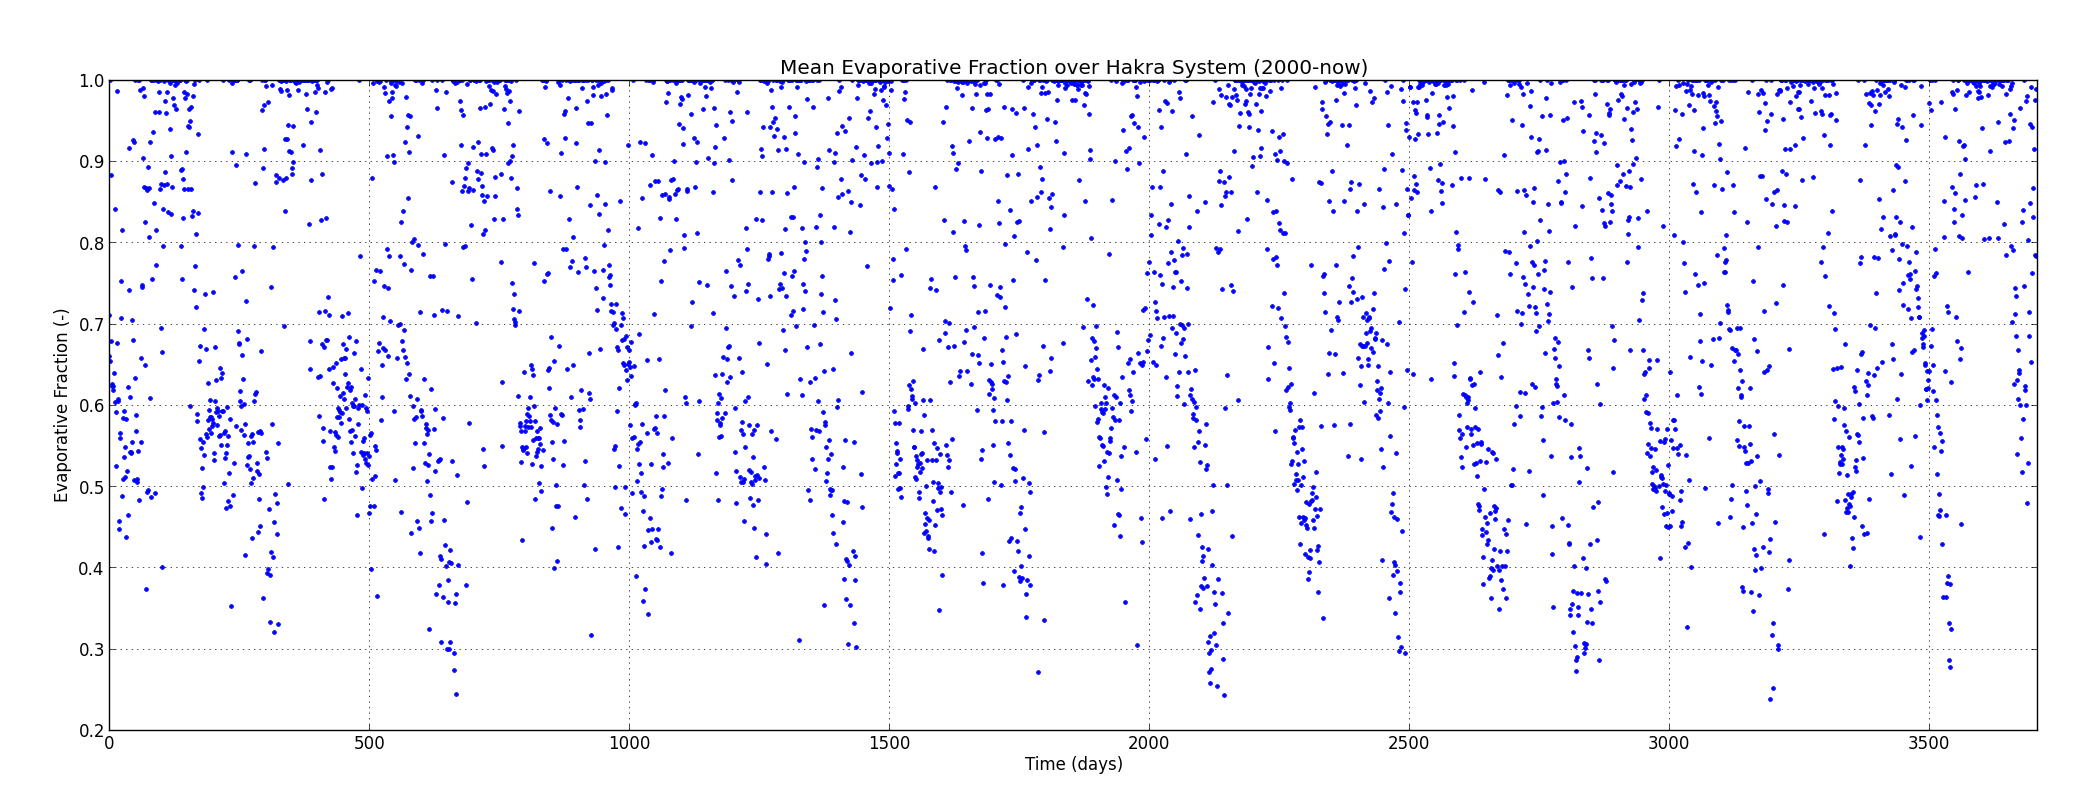
\includegraphics[width=8cm]{fess2012meaneftemporal}
\end{flushright}
\end{columns}
% Evaporative Fraction 2012 October 4th Hakra, Punjab, Pakistan ~4000 images (2000-2012)
\end{frame}

\subsection{Crop Water Consumption}
%%%%%%%%%%%%%%%%%%%%%%%%%%%%%%%%%%%%%%%%%%%%%%%%%%%%%%%%%%%%%%%%%%%%
\begin{frame}[fragile]{Crop water consumption in irrigation systems}

Actual evapotranspiration (mm/d, daily, 11 years)\\ 
for agricultural water performance management.\\
Irrigation System is 70,000 ha.

\begin{center}
 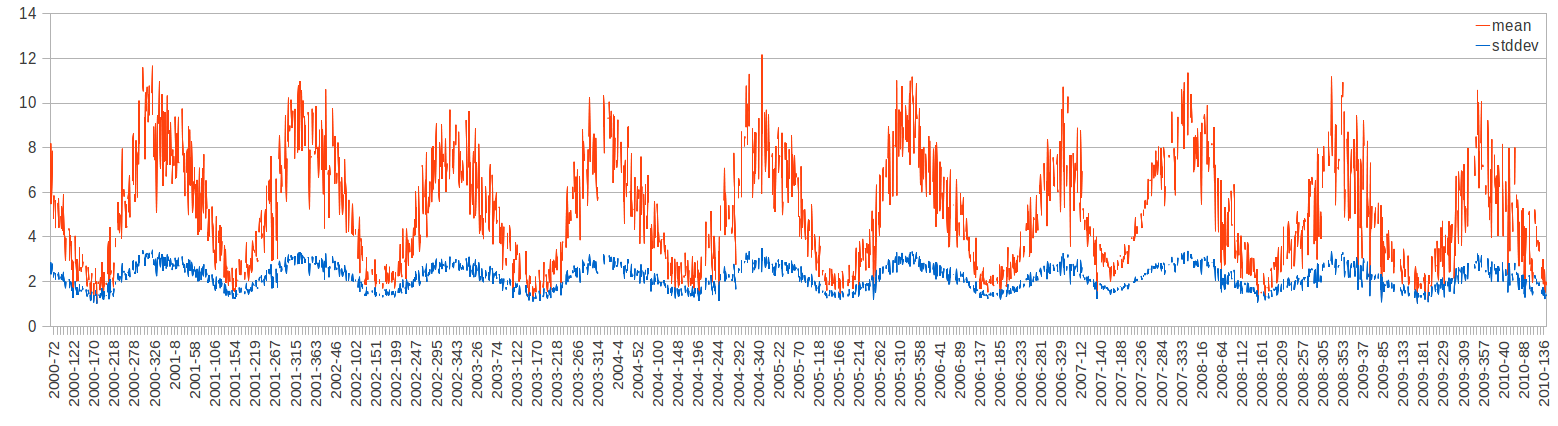
\includegraphics[width=11cm]{ciameanet}\\
 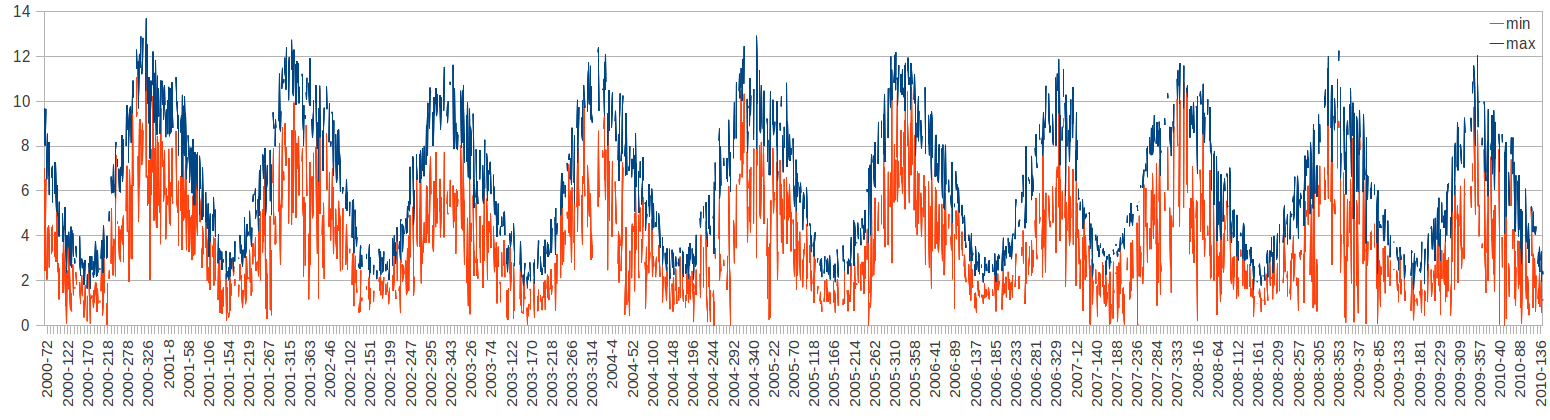
\includegraphics[width=11cm]{ciaminmaxet}
\end{center}
\end{frame}


%%%%%%%%%%%%%%%%%%%%%%%%%%%%%%%%%%%%%%%%%%%%%%%%%%%%%%%%%%%%%%%%%%%%
\begin{frame}[fragile]{}

\begin{center}
 {\Huge Code for} 
 \hspace{10mm} 
 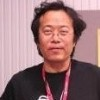
\includegraphics[width=3.5cm]{kayama}
\end{center}
\end{frame}

\subsection{River Basins Monitoring}
%%%%%%%%%%%%%%%%%%%%%%%%%%%%%%%%%%%%%%%%%%%%%%%%%%%%%%%%%%%%%%%%%%%%
\begin{frame}[fragile]{Water depletion in River Basins}

Actual evapotranspiration (mm/d, daily, 7 years)\\ 
for the Murray-Darling Basin (1M Km\textsuperscript{2})\\
Japan is 0.37M Km\textsuperscript{2}\\

\begin{center}
 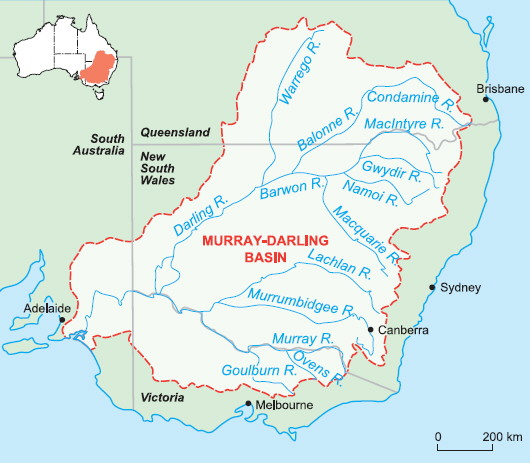
\includegraphics[width=6cm]{murray-darling_basin}
\end{center}
\end{frame}

%%%%%%%%%%%%%%%%%%%%%%%%%%%%%%%%%%%%%%%%%%%%%%%%%%%%%%%%%%%%%%%%%%%%
\begin{frame}[fragile]{Water depletion in River Basins}

Actual evapotranspiration (mm/d, daily, 7 years)\\ 
for the Murray-Darling Basin (1M Km\textsuperscript{2})\\
Japan is 0.37M Km\textsuperscript{2}\\

\begin{center}
 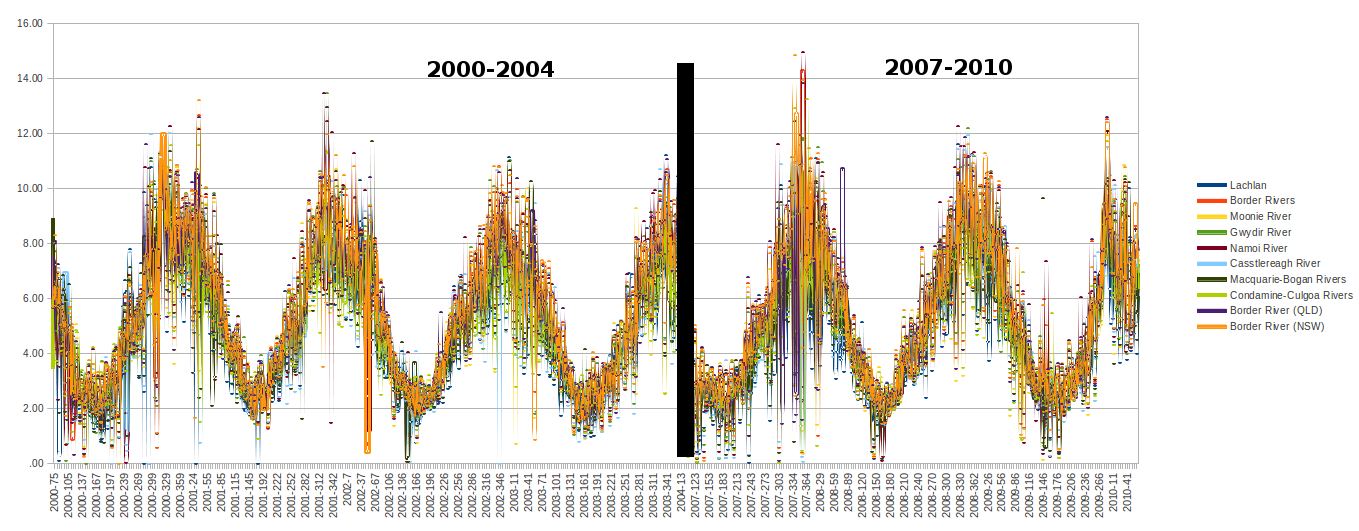
\includegraphics[width=11.5cm]{mdbmeanet}
\end{center}
\end{frame}

\subsection{Country Monitoring}
%%%%%%%%%%%%%%%%%%%%%%%%%%%%%%%%%%%%%%%%%%%%%%%%%%%%%%%%%%%%%%%%%%%%
\begin{frame}[fragile]{Evapotranspiration @ country level}

Actual evapotranspiration (365 days integrated)\\ 
for water resources monitoring \& management.\\

\begin{center}
 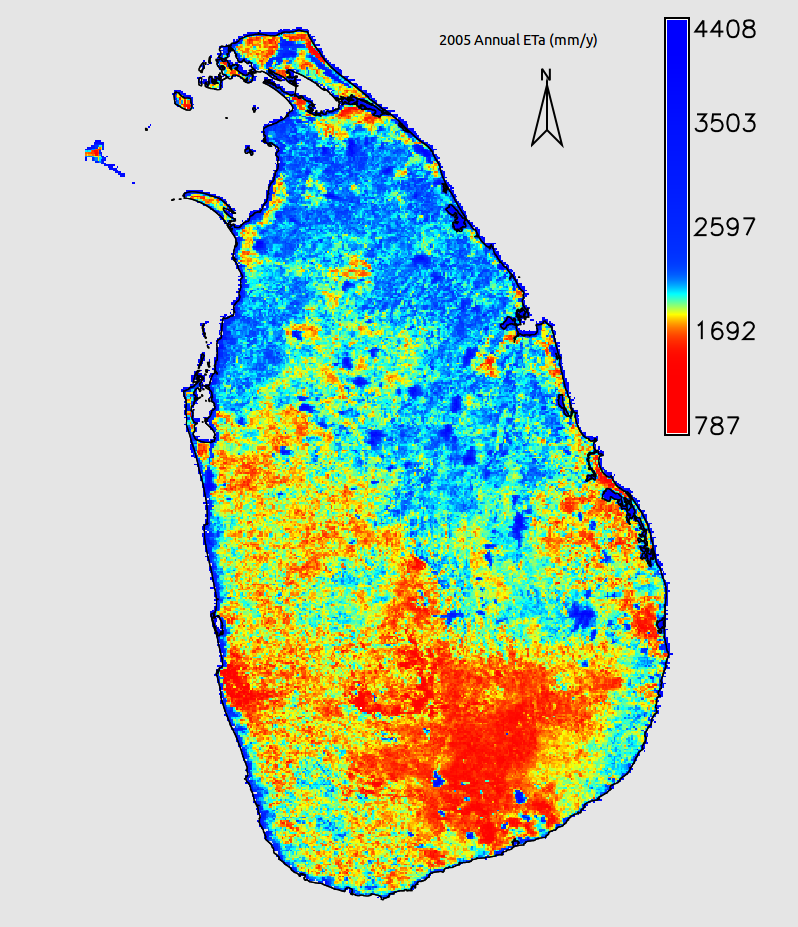
\includegraphics[width=5cm]{slet2005}
 \hspace{10mm}
 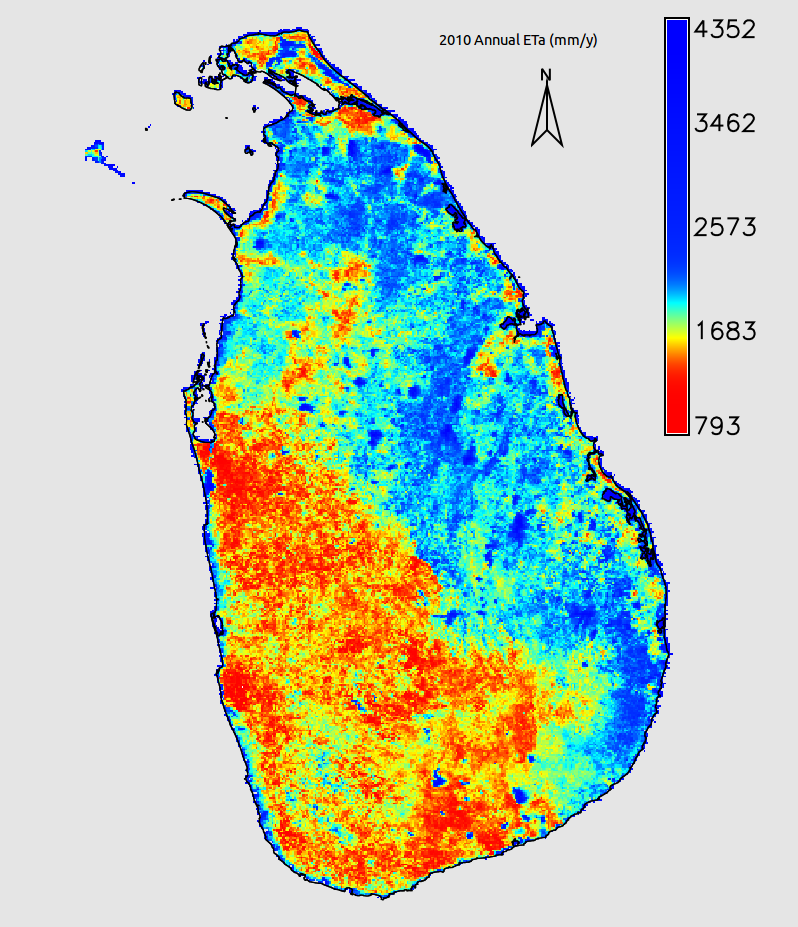
\includegraphics[width=5cm]{slet2010}
\end{center}
\end{frame}

\subsection{ET Models Benchmarking}
%%%%%%%%%%%%%%%%%%%%%%%%%%%%%%%%%%%%%%%%%%%%%%%%%%%%%%%%%%%%%%%%%%%%
\begin{frame}[fragile]{ET models Benchmarking}

\begin{center}
 Average ET for Sri Lanka, Daily 2000-2012 (mm/d, daily, 12.3 years)
 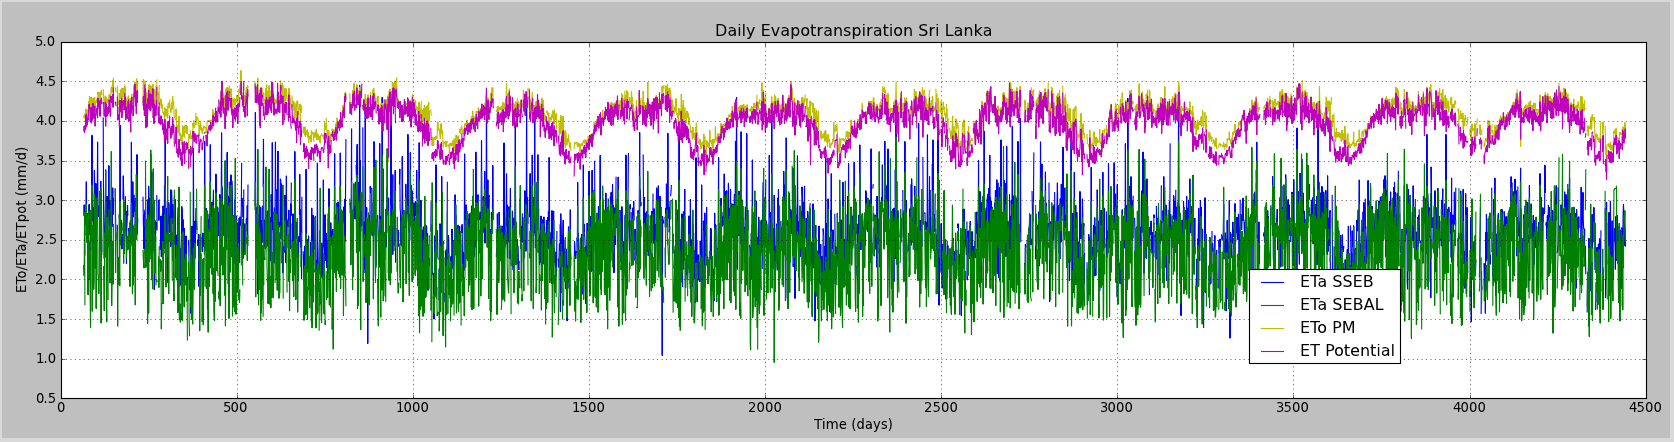
\includegraphics[width=12cm]{sltemporaletb}
\end{center}

\begin{block}{Comparison}
\begin{itemize}
 \item ETo \& ETpot (rad) are similar, expected.
 \item ETa models are not so similar, expected.
 \item ETo \& ETpot (rad) are higher than ETa models, expected.
\end{itemize}

\end{block}
\end{frame}


\section{Frameworks}
\subsection{Chain processing}
%%%%%%%%%%%%%%%%%%%%%%%%%%%%%%%%%%%%%%%%%%%%%%%%%%%%%%%%%%%%%%%%%%%%
\begin{frame}[fragile]{Chain processing}

Chain processing has a fundamental impact on remote sensing work:\\

\begin{itemize}
 \item Standardization limits bugs
 \item Less prone to human error
 \item Simpler parameterization access
 \item Permits to apply any number of modules to all target images
 \item Ensures maximum quality of generated images
\end{itemize}
\end{frame}

\subsection{Blueprint}
%%%%%%%%%%%%%%%%%%%%%%%%%%%%%%%%%%%%%%%%%%%%%%%%%%%%%%%%%%%%%%%%%%%%
\begin{frame}[fragile]{Blueprint}

\begin{center}
 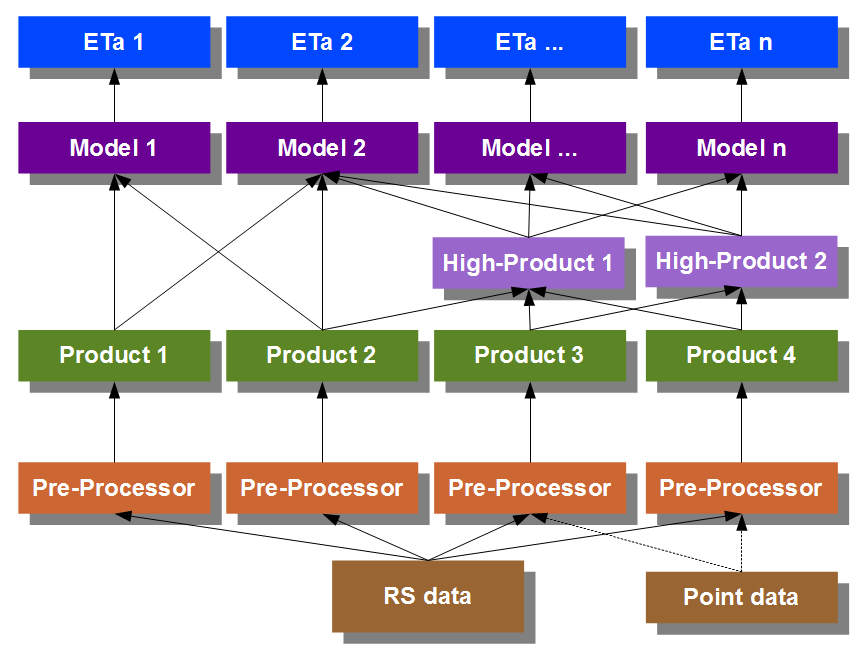
\includegraphics[width=7.5cm]{chain0}
\end{center}

\begin{itemize}
 \item GDAL+[C+OpenMP]
 \item GRASSGIS+pyGRASS+[C+OpenMP]
\end{itemize}
\end{frame}

\subsection{GDAL}
%%%%%%%%%%%%%%%%%%%%%%%%%%%%%%%%%%%%%%%%%%%%%%%%%%%%%%%%%%%%%%%%%%%%
\begin{frame}[fragile]{GDAL framework}

\begin{center}
 GDAL+[C+OpenMP]
 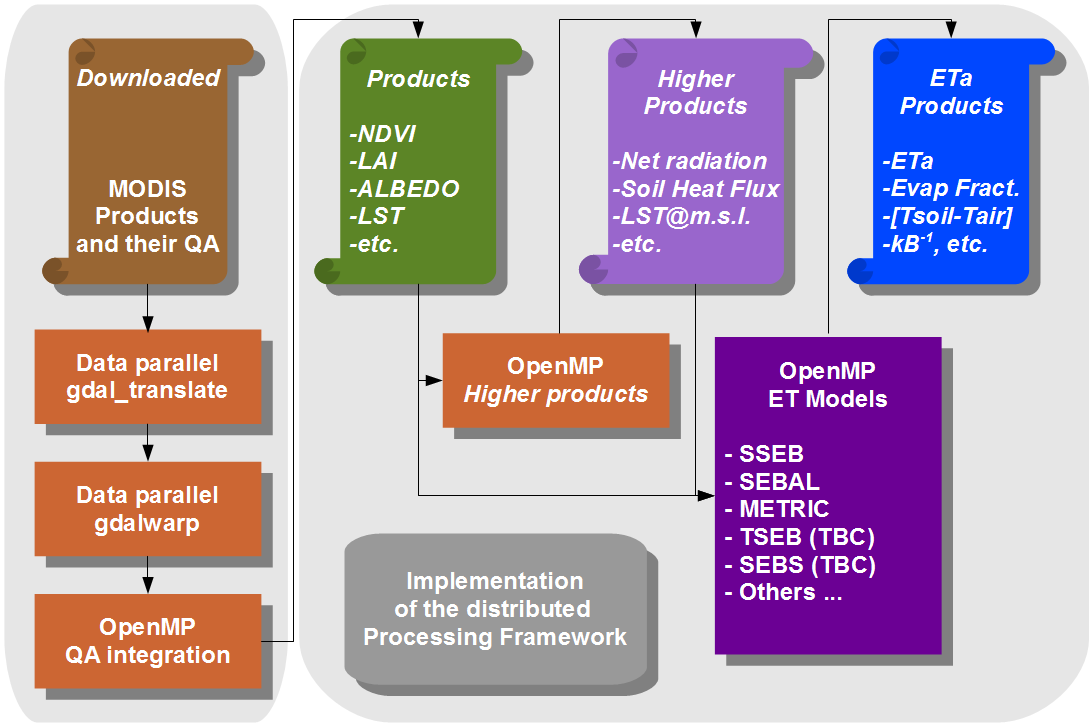
\includegraphics[width=8.5cm]{chain2}
\end{center}
\end{frame}

%%%%%%%%%%%%%%%%%%%%%%%%%%%%%%%%%%%%%%%%%%%%%%%%%%%%%%%%%%%%%%%%%%%%
\begin{frame}[fragile]{GDAL framework}

\begin{columns}[l]
\column[t]{0.6\textwidth}
\begin{center}
 OpenMP Distribution \\
 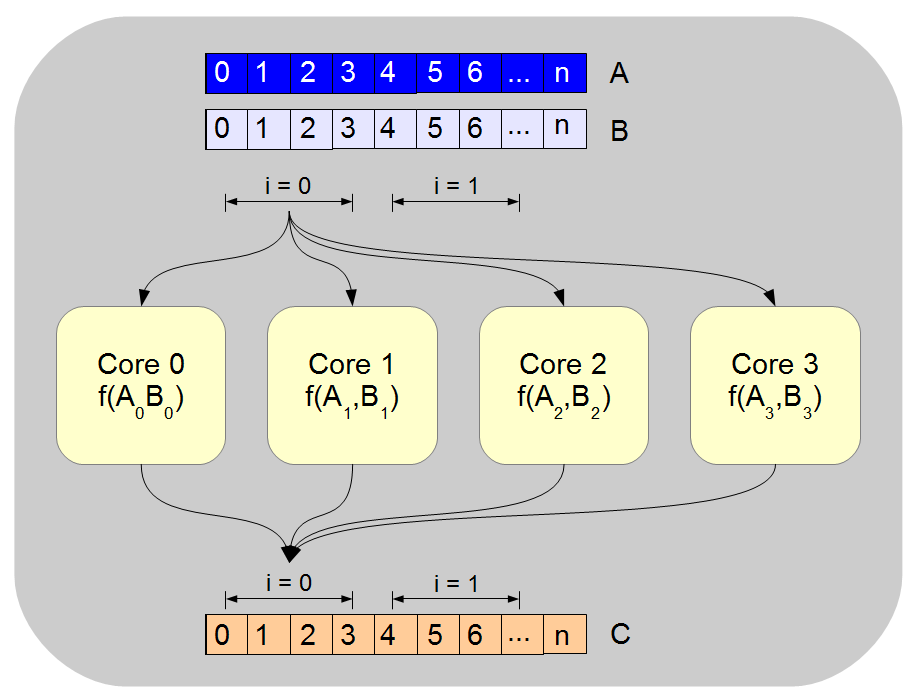
\includegraphics[width=7.5cm]{chain1}
\end{center}
\column[t]{0.4\textwidth}
\begin{center}
 Cores \\
 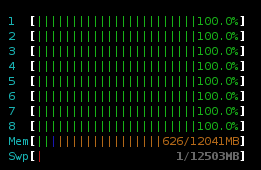
\includegraphics[width=4cm]{cores}
\end{center}
\end{columns}
\end{frame}


\subsection{GRASS GIS}
%%%%%%%%%%%%%%%%%%%%%%%%%%%%%%%%%%%%%%%%%%%%%%%%%%%%%%%%%%%%%%%%%%%%
\begin{frame}[fragile]{GRASS GIS framework}

\begin{center}
 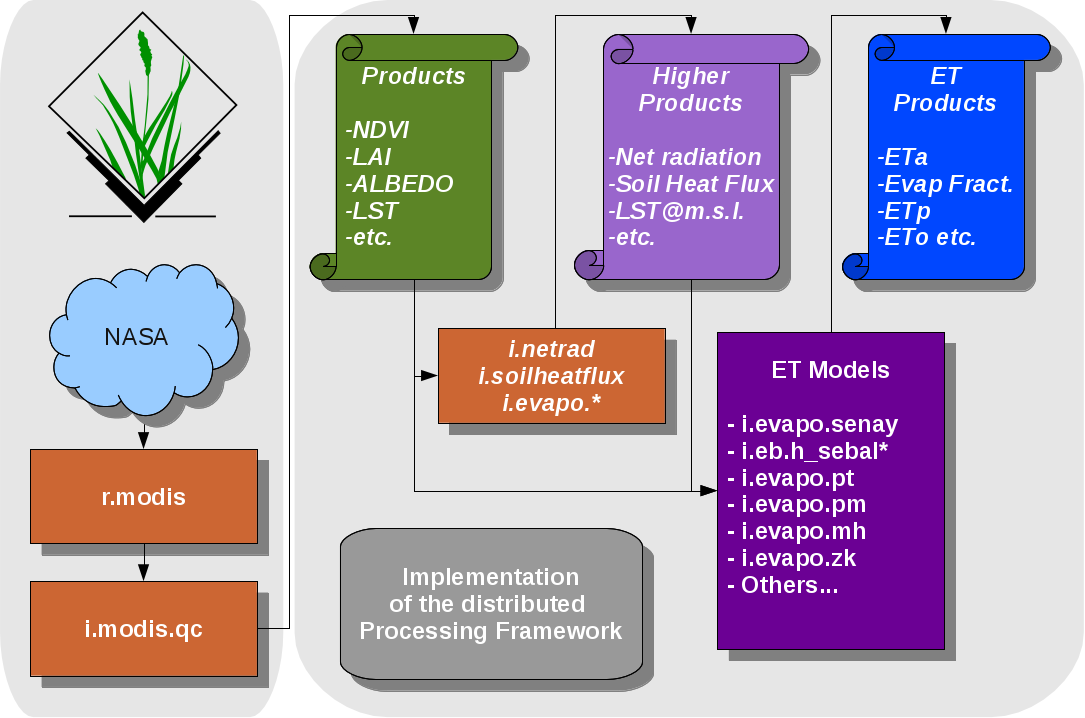
\includegraphics[width=8.5cm]{architecture_implementation}
\end{center}

\begin{block}{metaModule concept}
{\bf pyGRASS:} vertical integration of GRASS GIS modules\\
{\bf GRASS GIS modules:} [C+OpenMP]
\end{block}

\end{frame}

%%%%%%%%%%%%%%%%%%%%%%%%%%%%%%%%%%%%%%%%%%%%%%%%%%%%%%%%%%%%%%%%%%%%
\begin{frame}[fragile]{pyGRASS}

\begin{center}
 Summary for Landsat 7 pyGRASS MetaModule
 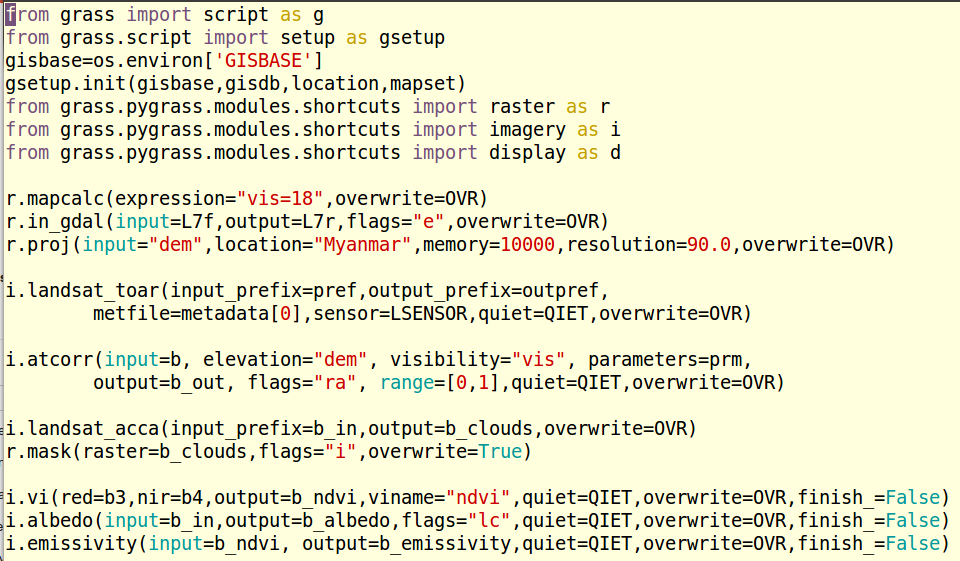
\includegraphics[width=10cm]{pyGRASS1}\\
 \href{http://grasswiki.osgeo.org/wiki/Python/pygrass}{http://grasswiki.osgeo.org/wiki/Python/pygrass}
\end{center}

\end{frame}

\section{Future}
%%%%%%%%%%%%%%%%%%%%%%%%%%%%%%%%%%%%%%%%%%%%%%%%%%%%%%%%%%%%%%%%%%%%
\begin{frame}[fragile]{Future: 128-cores from Tile-GX}

\begin{columns}[l]
\column[t]{0.5\textwidth}
\begin{center}
 64-core Tile-GX\newline\linebreak
 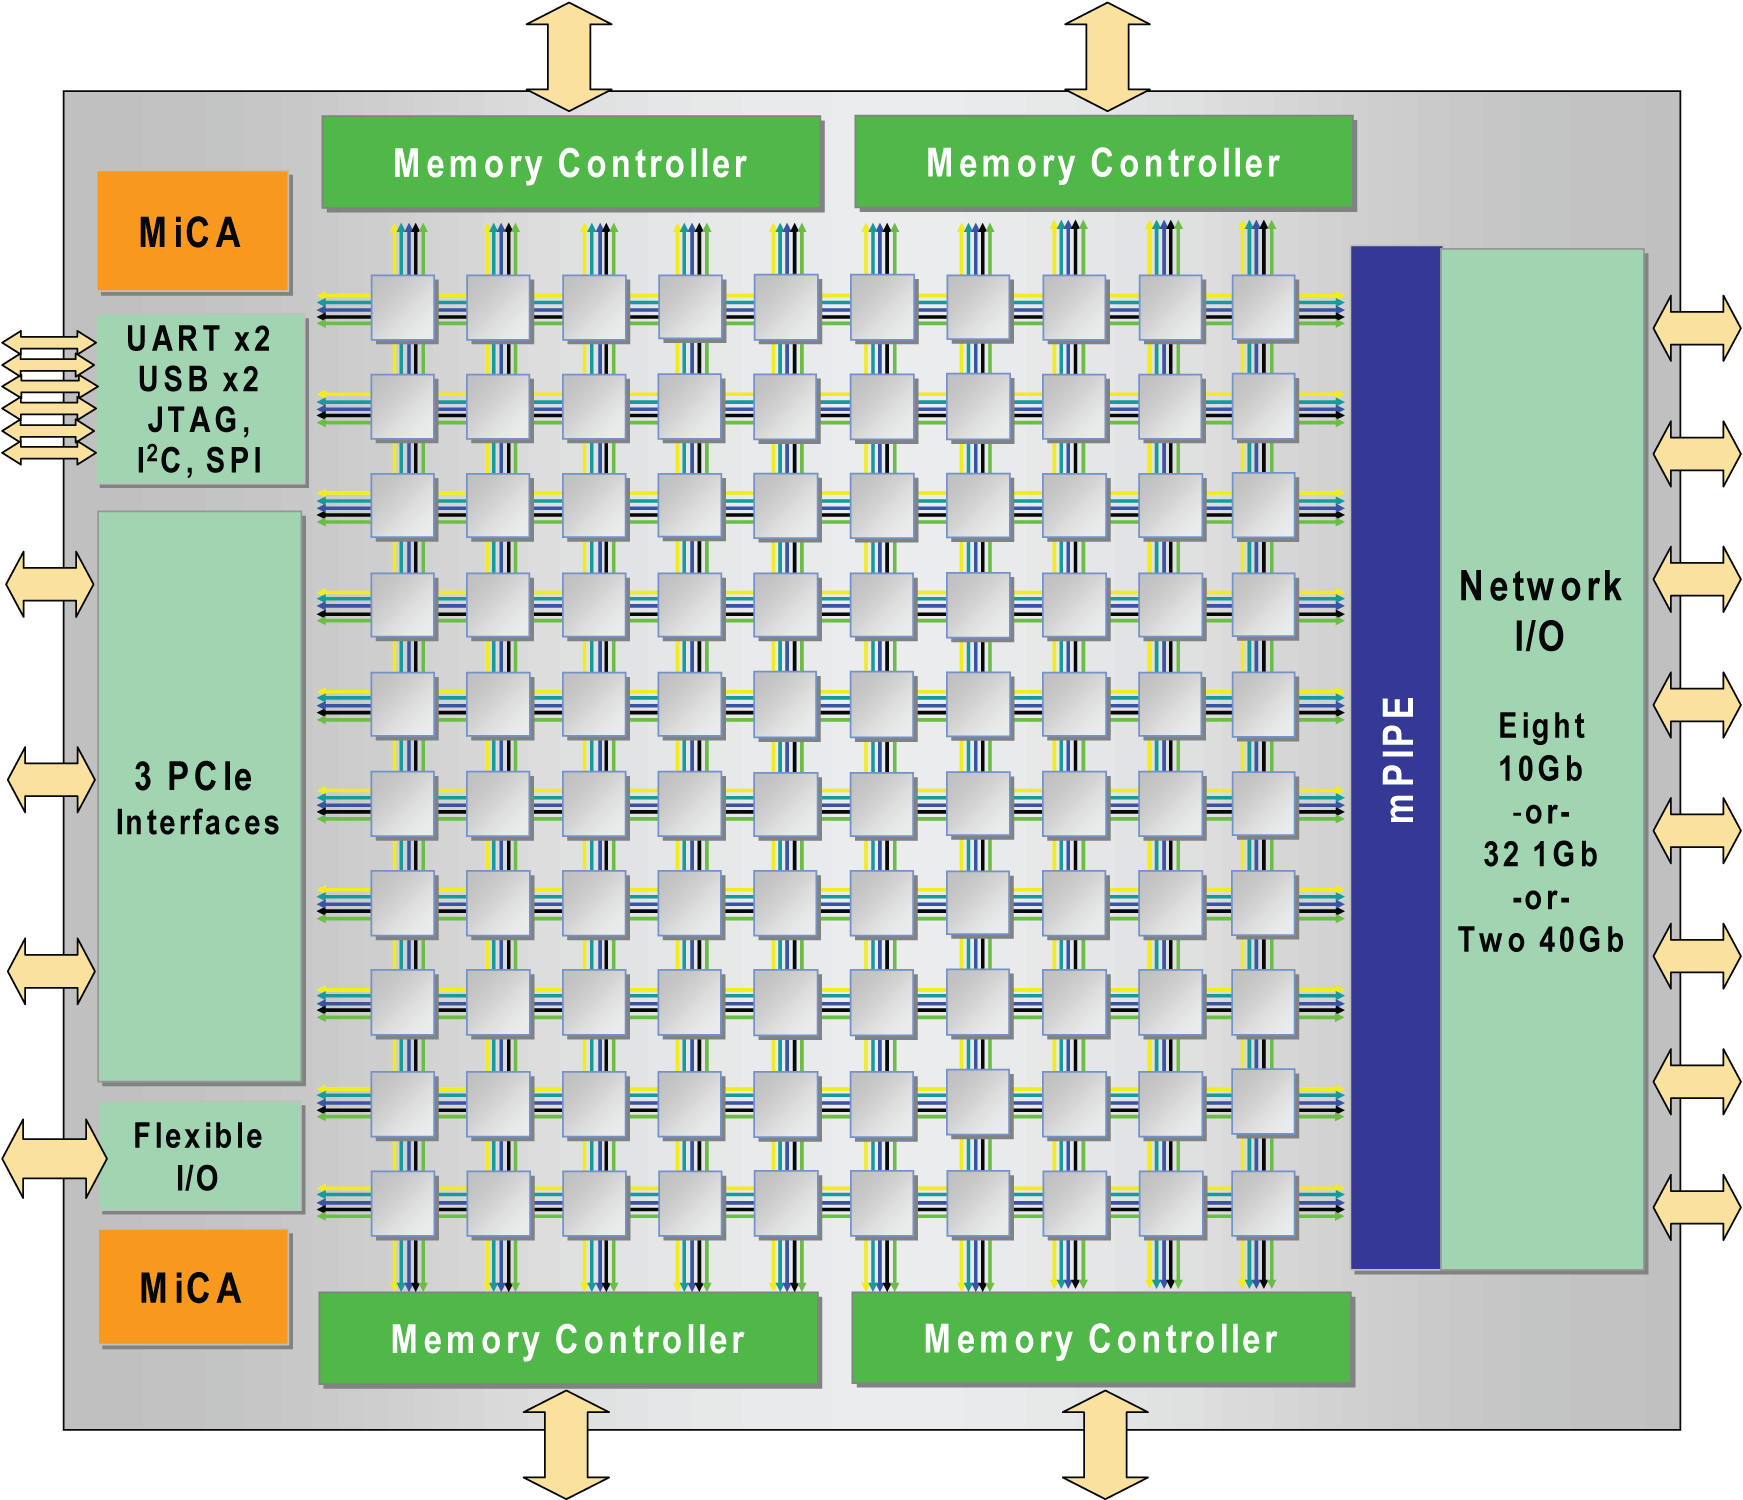
\includegraphics[width=5cm]{TILE-Gx_Block_Diagram_large}
\end{center}
\column[t]{0.5\textwidth}
\begin{center}
 Dual Tile-GX on {\small $1/2$} rack board\newline\linebreak
 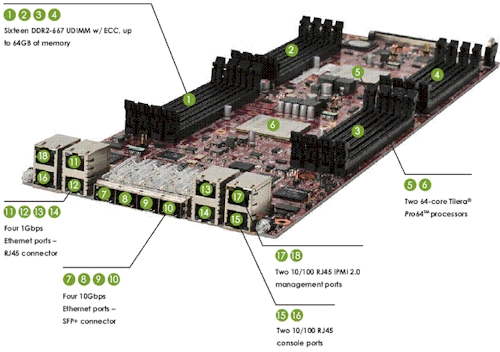
\includegraphics[width=5cm]{tilera_quanta_sq2_mobo}
\end{center}

\end{columns}

\end{frame}

%%%%%%%%%%%%%%%%%%%%%%%%%%%%%%%%%%%%%%%%%%%%%%%%%%%%%%%%%%%%%%%%%%%%
\begin{frame}[fragile]{Future: 120-cores from Xeon Phi}

\begin{columns}[l]
\column[t]{0.5\textwidth}
\begin{center}
 60-core Phi\newline\linebreak
 \includegraphics[width=5cm]{xeon-phi-oh}
\end{center}
\column[t]{0.5\textwidth}
\begin{center}
 Dual Phi in Gygabyte cage\newline\linebreak
 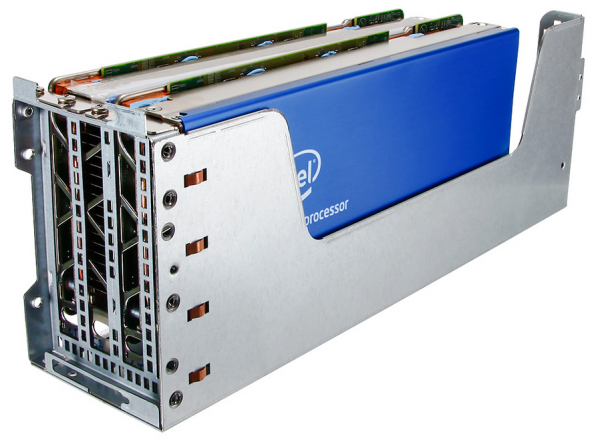
\includegraphics[width=5cm]{Gigabyte-GS-R22PHL-Xeon-Phi-Cage-600x440}
\end{center}

\end{columns}

\end{frame}

%%%%%%%%%%%%%%%%%%%%%%%%%%%%%%%%%%%%%%%%%%%%%%%%%%%%%%%%%%%%%%%%%%%%
\begin{frame}[fragile]{Outlooks}

\begin{itemize}
 \item Multi-Cores Hardware (Tile-GX, Xeon Phi)
 \item Multi-GPU distribution (OpenCL, CUDA)
 \item Multi-CPU distribution (MPI)
 \item MODIS and Landsat archives under close pipe distance?
 \item Online: automatic, PyWPS, SOS/network ? 
\end{itemize}

\end{frame}

\section{Conclusions}
%%%%%%%%%%%%%%%%%%%%%%%%%%%%%%%%%%%%%%%%%%%%%%%%%%%%%%%%%%%%%%%%%%%%
\begin{frame}[fragile]{Conclusions}

\begin{block}{Distributed ET models benchmarking setup with OSGEO tools}
\begin{itemize}
 \item {\bf GDAL:} C+OpenMP
 \item {\bf GDAL:} Core-based scaling
 \item {\bf GRASS GIS:} pyGRASS for metaModule
 \item {\bf GRASS GIS:} pyGRASS finish\_=False
 \item {\bf GRASS GIS:} C+OpenMP inside modules
 \item {\bf Targets:} MODIS (Terra/Aqua), Landsat (all), Aster
\end{itemize}
\end{block}

\end{frame}

% \section{Collaboration Call}
%%%%%%%%%%%%%%%%%%%%%%%%%%%%%%%%%%%%%%%%%%%%%%%%%%%%%%%%%%%%%%%%%%%%
\begin{frame}[fragile]{Collaboration call}

We are looking for collaborators:
\begin{itemize}
 \item Having HPC capabilities
 \item Interested in Global Water ET monitoring from Space
 \item Using distributed FOSS4G tools
\end{itemize}

\end{frame}

%%%%%%%%%%%%%%%%%%%%%%%%%%%%%%%%%%%%%%%%%%%%%%%%%%%%%%%%%%%%%%%%%%%%

%%%%%%%%%%%%%%%%%%%%%%%%%%%%%%%%%%%%%%%%%%%%%%%%%%%%%%%%%%%%%%%%%%%%
\begin{frame}[fragile]{Thank You}

\vspace{50mm}
\begin{flushright}
 
\includegraphics[width=3cm]{iwmi}
 \hspace{10mm}
 
\includegraphics[width=2cm]{etb_qr}
\end{flushright}

\end{frame}

\end{document}
